\chapter{Les structures arborescentes}
\minitoc
Nous allons voir deux types d'arbres : 
\begin{enumerate}
	\item L'arbre GRD : << Gauche Racine Droite >>
	\item Les arbres rouges noirs
\end{enumerate}
Ce sont des arbres binaires: chaque noeud de l'arbre à au lu deux fils. 
\attention{Les informations sont rangés dans l'arbre en respectant un certain critère}
\section{L'arbre GRD : <<Gauche Racine Droite>>}
	\subsection{Critère de rangement}
	Quelque soit le noeud de l'arbre : 
	\begin{itemize}
		\item les informations rangées à gauche de la racine de ce noeud sont inférieur ou égal à cette racine.
		\item les informations rangées à droite de la racine de ce noeud sont supérieur à cette racine.
	\end{itemize}
\begin{figure}[H]
\centering
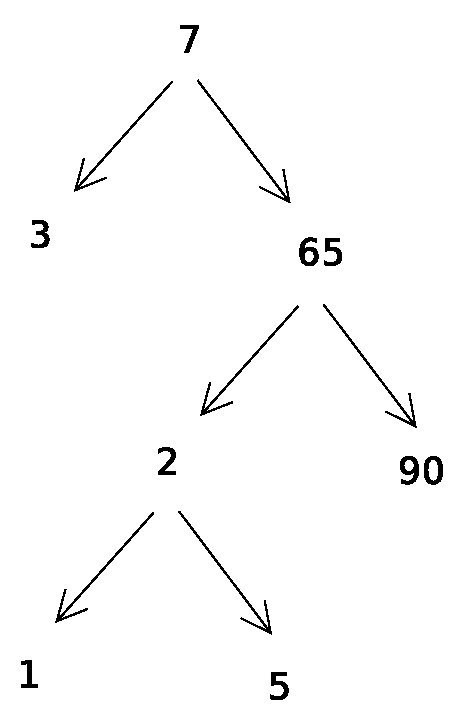
\includegraphics[width=6cm]{content/schemas/arbresGRB.eps}
\caption{Arbre GRB}
\end{figure}
	\subsection{Implémentation du TAD}
\begin{figure}[H]
\centering
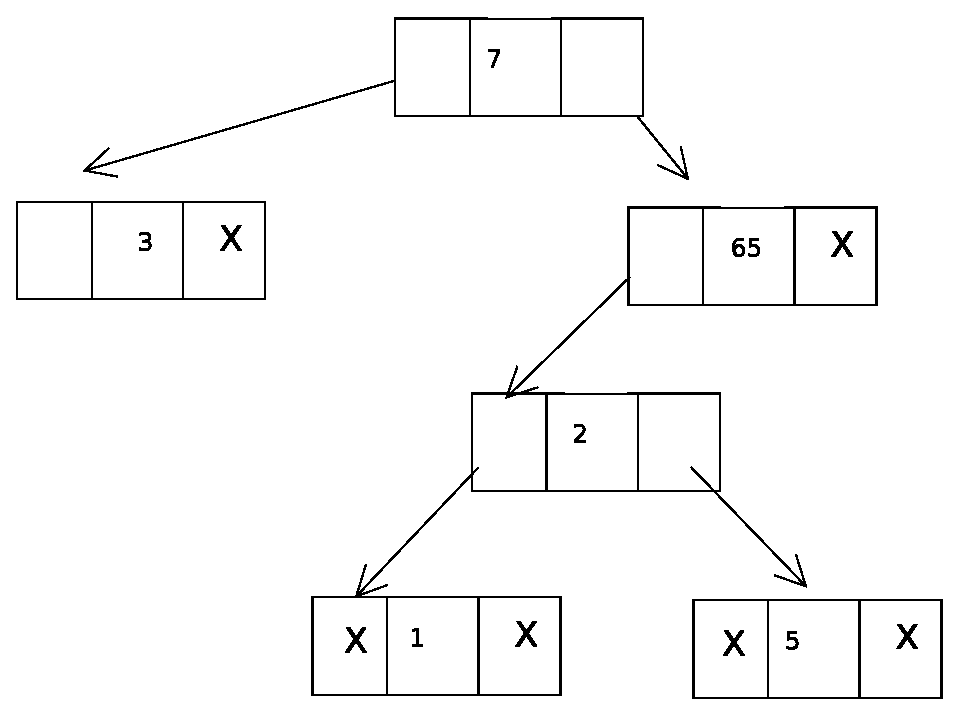
\includegraphics[width=10cm]{content/schemas/arbresGRBImplementation.eps}
\caption{Implémentation de l'arbre GRB}
\end{figure}
\lstinputlisting[language=C, caption=Arbre GRD -- Header]{content/code/arbreGRB.h}
\lstinputlisting[language=C, caption=Arbre GRD -- Implémentation]{content/code/arbreGRB.c}
\section{Les arbres rouges noirs}
